\documentclass[a4paper, 14pt]{extarticle}

% Поля
%--------------------------------------
\usepackage{geometry}
\geometry{a4paper,tmargin=2cm,bmargin=2cm,lmargin=3cm,rmargin=1cm}
%--------------------------------------


%Russian-specific packages
%--------------------------------------
\usepackage[T2A]{fontenc}
\usepackage[utf8]{inputenc} 
\usepackage[english, main=russian]{babel}
%--------------------------------------

\usepackage{textcomp}

% Красная строка
%--------------------------------------
\usepackage{indentfirst}               
%--------------------------------------             


%Graphics
%--------------------------------------
\usepackage{graphicx}
\graphicspath{ {./images/} }
\usepackage{wrapfig}
%--------------------------------------

% Полуторный интервал
%--------------------------------------
\linespread{1.3}                    
%--------------------------------------

%Выравнивание и переносы
%--------------------------------------
% Избавляемся от переполнений
\sloppy
% Запрещаем разрыв страницы после первой строки абзаца
\clubpenalty=10000
% Запрещаем разрыв страницы после последней строки абзаца
\widowpenalty=10000
%--------------------------------------

%Списки
\usepackage{enumitem}

%Подписи
\usepackage{caption} 

%Гиперссылки
\usepackage{hyperref}

\hypersetup {
	unicode=true
}

%Рисунки
%--------------------------------------
\DeclareCaptionLabelSeparator*{emdash}{~--- }
\captionsetup[figure]{labelsep=emdash,font=onehalfspacing,position=bottom}
%--------------------------------------

\usepackage{tempora}

%Листинги
%--------------------------------------
\usepackage{listings}
\lstset{
  basicstyle=\ttfamily\footnotesize, 
  %basicstyle=\footnotesize\AnkaCoder,        % the size of the fonts that are used for the code
  breakatwhitespace=false,         % sets if automatic breaks shoulbd only happen at whitespace
  breaklines=true,                 % sets automatic line breaking
  captionpos=t,                    % sets the caption-position to bottom
  inputencoding=utf8,
  frame=single,                    % adds a frame around the code
  keepspaces=true,                 % keeps spaces in text, useful for keeping indentation of code (possibly needs columns=flexible)
  keywordstyle=\bf,       % keyword style
  numbers=left,                    % where to put the line-numbers; possible values are (none, left, right)
  numbersep=5pt,                   % how far the line-numbers are from the code
  xleftmargin=25pt,
  xrightmargin=25pt,
  showspaces=false,                % show spaces everywhere adding particular underscores; it overrides 'showstringspaces'
  showstringspaces=false,          % underline spaces within strings only
  showtabs=false,                  % show tabs within strings adding particular underscores
  stepnumber=1,                    % the step between two line-numbers. If it's 1, each line will be numbered
  tabsize=2,                       % sets default tabsize to 8 spaces
  title=\lstname                   % show the filename of files included with \lstinputlisting; also try caption instead of title
}
%--------------------------------------

%%% Математические пакеты %%%
%--------------------------------------
\usepackage{amsthm,amsfonts,amsmath,amssymb,amscd}  % Математические дополнения от AMS
\usepackage{mathtools}                              % Добавляет окружение multlined
\usepackage[perpage]{footmisc}
%--------------------------------------

%--------------------------------------
%			НАЧАЛО ДОКУМЕНТА
%--------------------------------------

\begin{document}

%--------------------------------------
%			ТИТУЛЬНЫЙ ЛИСТ
%--------------------------------------
\begin{titlepage}
\thispagestyle{empty}
\newpage


%Шапка титульного листа
%--------------------------------------
\vspace*{-60pt}
\hspace{-65pt}
\begin{minipage}{0.3\textwidth}
\hspace*{-20pt}\centering

\includegraphics[width=\textwidth]{emblem}
\end{minipage}
\begin{minipage}{0.67\textwidth}\small \textbf{
\vspace*{-0.7ex}
\hspace*{-6pt}\centerline{Министерство науки и высшего образования Российской Федерации}
\vspace*{-0.7ex}
\centerline{Федеральное государственное бюджетное образовательное учреждение }
\vspace*{-0.7ex}
\centerline{высшего образования}
\vspace*{-0.7ex}
\centerline{<<Московский государственный технический университет}
\vspace*{-0.7ex}
\centerline{имени Н.Э. Баумана}
\vspace*{-0.7ex}
\centerline{(национальный исследовательский университет)>>}
\vspace*{-0.7ex}
\centerline{(МГТУ им. Н.Э. Баумана)}}
\end{minipage}
%--------------------------------------

%Полосы
%--------------------------------------
\vspace{-25pt}
\hspace{-35pt}\rule{\textwidth}{2.3pt}

\vspace*{-20.3pt}
\hspace{-35pt}\rule{\textwidth}{0.4pt}
%--------------------------------------

\vspace{1.5ex}
\hspace{-35pt} \noindent \small ФАКУЛЬТЕТ\hspace{80pt} <<Информатика и системы управления>>

\vspace*{-16pt}
\hspace{47pt}\rule{0.83\textwidth}{0.4pt}

\vspace{0.5ex}
\hspace{-35pt} \noindent \small КАФЕДРА\hspace{50pt} <<Теоретическая информатика и компьютерные технологии>>

\vspace*{-16pt}
\hspace{30pt}\rule{0.866\textwidth}{0.4pt}
  
\vspace{11em}

\begin{center}
\Large {\bf Лабораторная работа № 3} \\
\large {\bf по курсу <<Разработка мобильных приложений>>} \\
\large <<Проверка усвоенного материала по теме использования библиотек  работы с 3D объектами>>
\end{center}\normalsize

\vspace{8em}


\begin{flushright}
  {Студентка группы ИУ9-72Б Самохвалова П. С. \hspace*{15pt}\\
  \vspace{2ex}
  Преподаватель Посевин Д. П.\hspace*{15pt}}
\end{flushright}

\bigskip

\vfill
 

\begin{center}
\textsl{Москва 2023}
\end{center}
\end{titlepage}
%--------------------------------------
%		КОНЕЦ ТИТУЛЬНОГО ЛИСТА
%--------------------------------------

\renewcommand{\ttdefault}{pcr}

\setlength{\tabcolsep}{3pt}
\newpage
\setcounter{page}{2}

\section{Задание}\label{Sect::task}

Реализовать  мобильное приложение выводящее трехмерный объект по вариантам. Использование библиотеки на усмотрение программиста из рассмотренных на лекции.

Индивидуальный вариант

Реализовать приложение моделирования движения глаз человека влево и вправо, модель головы человека можно взять из лекции. Движение глаз реализовывается ползунком. Голова должна вращаться.

\section{Практическая реализация}\label{Sect::code}

Исходный код программы представлен в листинге~\ref{lst:code1}.

\begin{lstlisting}[language={},caption={Работа с трехмерными объектами},label={lst:code1}]
import 'package:flutter/material.dart';
import 'package:flutter_cube/flutter_cube.dart';

void main() => runApp(MyApp());

class MyApp extends StatelessWidget {
  @override
  Widget build(BuildContext context) {
    return MaterialApp(
      title: 'Flutter Cube',
      theme: ThemeData.dark(),
      home: MyHomePage(title: 'Flutter Cube Home Page'),
    );
  }
}

class MyHomePage extends StatefulWidget {
  MyHomePage({Key? key, this.title}) : super(key: key);

  final String? title;

  @override
  _MyHomePageState createState() => _MyHomePageState();
}

class _MyHomePageState extends State<MyHomePage> with SingleTickerProviderStateMixin {
  late Scene _scene;
  Object? _bunny;
  Object? _eyes;
  late AnimationController _controller;
  double _ambient = 0.1;
  double _diffuse = 0.8;
  double _specular = 0.5;
  double _shininess = 0.0;

  double x1 = 0.0;
  double y1 = 0.0;

  final Object cube1 = Object(
    scale: Vector3(0.5, 0.5, 0.5),
    position: Vector3(0.2, 0.9, 0.5)..scale(3),
    lighting: true,
    fileName: 'assets/eyeball/eyeball.obj',
  );

  final Object cube2 = Object(
    scale: Vector3(0.5, 0.5, 0.5),
    position: Vector3(-0.2, 0.9, 0.5)..scale(3),
    lighting: true,
    fileName: 'assets/eyeball/eyeball.obj',
  );

  void _onSceneCreated(Scene scene) {
    _scene = scene;
    scene.camera.position.z = 10;
    scene.light.position.setFrom(Vector3(0, 10, 10));
    // scene.light.setColor(Colors.white, _ambient, _diffuse, _specular);
    _bunny = Object(position: Vector3(0, 0.0, 0), scale: Vector3(10.0, 10.0, 10.0), lighting: true, fileName: 'assets/face/face.obj');
    _eyes = Object();
    _eyes!.add(cube1);
    _eyes!.add(cube2);

    _bunny!.lighting = true;
    _eyes!.lighting = false;

    scene.world.add(_bunny!);
    scene.world.add(_eyes!);
  }

  @override
  void initState() {
    super.initState();
    _controller = AnimationController(duration: Duration(milliseconds: 30000), vsync: this)
      ..addListener(() {
        // if (_bunny != null) {
        //   _bunny!.rotation.y = _controller.value * 360;
        //   _bunny!.updateTransform();
        //   _scene.update();
        // }
        //
        // if (_eyes != null) {
        //   _eyes!.rotation.y = _controller.value * 360;
        //   _eyes!.updateTransform();
        //   _scene.update();
        // }
      })
      ..repeat();
  }

  @override
  void dispose() {
    _controller.dispose();
    super.dispose();
  }

  @override
  Widget build(BuildContext context) {
    return Scaffold(
      appBar: AppBar(
        title: Text(widget.title!),
      ),
      body: Stack(
        children: <Widget>[
          Cube(onSceneCreated: _onSceneCreated),
          Column(
            mainAxisAlignment: MainAxisAlignment.end,
            children: <Widget>[
              Row(
                mainAxisAlignment: MainAxisAlignment.end,
                children: <Widget>[
                  Flexible(flex: 2, child: Text('diffuse')),
                  Flexible(
                    flex: 8,
                    child: Slider(
                      value: _diffuse,
                      min: 0.0,
                      max: 1.0,
                      divisions: 100,
                      onChanged: (value) {
                        setState(() {
                          _diffuse = value;
                          _scene.light.setColor(Colors.white, _ambient, _diffuse, _specular);
                        });
                      },
                    ),
                  ),
                ],
              ),
              Row(
                mainAxisAlignment: MainAxisAlignment.end,
                children: <Widget>[
                  Flexible(flex: 2, child: Text('Eye rotation up and down')),
                  Flexible(
                    flex: 8,
                    child: Slider(
                      value: x1,
                      min: -45.0,
                      max: 45.0,
                      // divisions: 32,
                      onChanged: (value) {
                        setState(() {
                          x1 = value;
                          cube1.rotation.x = x1;
                          cube1.updateTransform();
                          cube2.rotation.x = x1;
                          cube2.updateTransform();
                        });
                      },
                    ),
                    // child: Slider(
                    //   value: _specular,
                    //   min: 0.0,
                    //   max: 1.0,
                    //   divisions: 100,
                    //   onChanged: (value) {
                    //     setState(() {
                    //       _specular = value;
                    //       _scene.light.setColor(Colors.white, _ambient, _diffuse, _specular);
                    //     });
                    //   },
                    // ),
                  ),
                ],
              ),
              Row(
                mainAxisAlignment: MainAxisAlignment.end,
                children: <Widget>[
                  Flexible(flex: 2, child: Text('Eye rotation left and right')),
                  Flexible(
                    flex: 8,
                    child: Slider(
                      value: y1,
                      min: -45.0,
                      max: 45.0,
                      // divisions: 32,
                      onChanged: (value) {
                        setState(() {
                          y1 = value;
                          cube1.rotation.y = y1;
                          cube1.updateTransform();
                          cube2.rotation.y = y1;
                          cube2.updateTransform();
                        });
                      },
                    ),
                    // child: Slider(
                    //   value: _shininess,
                    //   min: 0.0,
                    //   max: 32.0,
                    //   divisions: 32,
                    //   onChanged: (value) {
                    //     setState(() {
                    //       _shininess = value;
                    //       _bunny!.mesh.material.shininess = _shininess;
                    //       _eyes!.mesh.material.shininess = _shininess;
                    //     });
                    //   },
                    // ),
                  ),
                ],
              ),
            ],
          ),
        ],
      ),
    );
  }
}

\end{lstlisting}

\section{Результаты}\label{Sect::res}

Результаты работы программы представлены на рисунках~\ref{fig:img1}~--~\ref{fig:img4}.  

\begin{figure}[!htb]
	\centering
	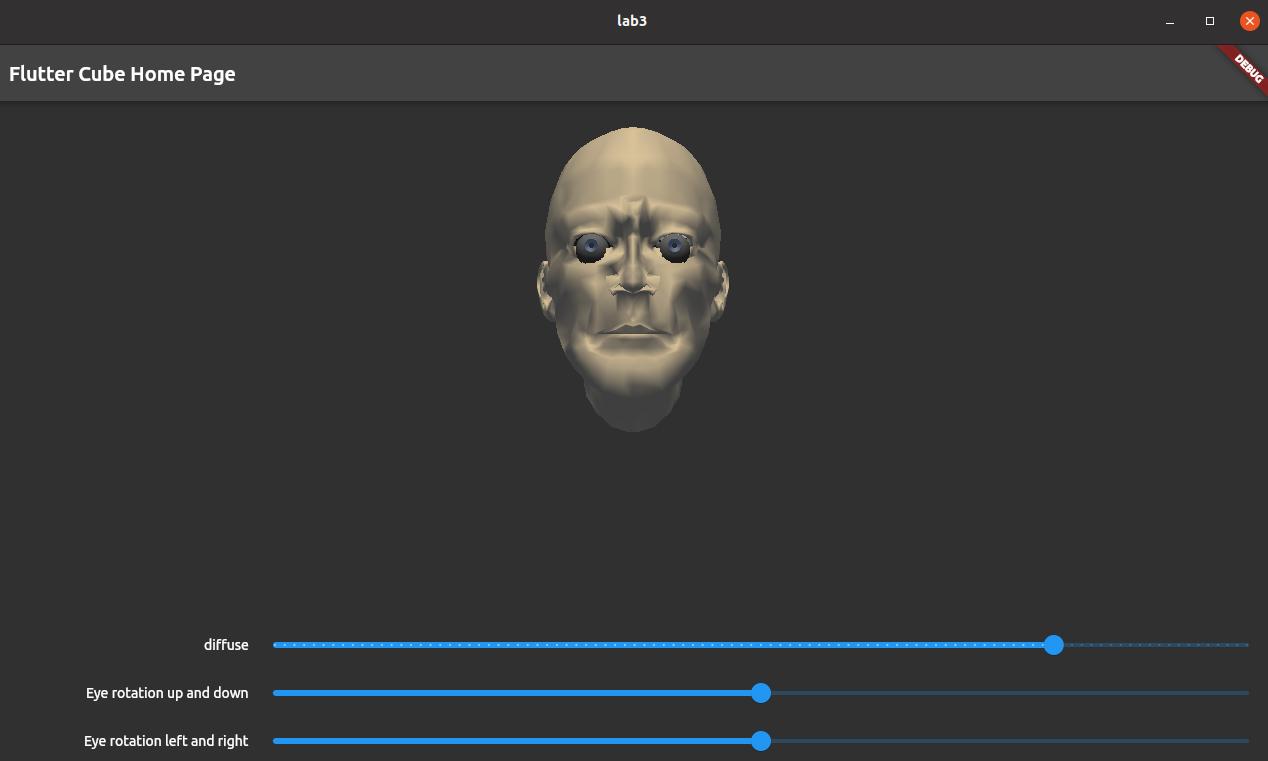
\includegraphics[width=0.8\textwidth]{img1}
\caption{Приложение}
\label{fig:img1}
\end{figure}

\begin{figure}[!htb]
	\centering
	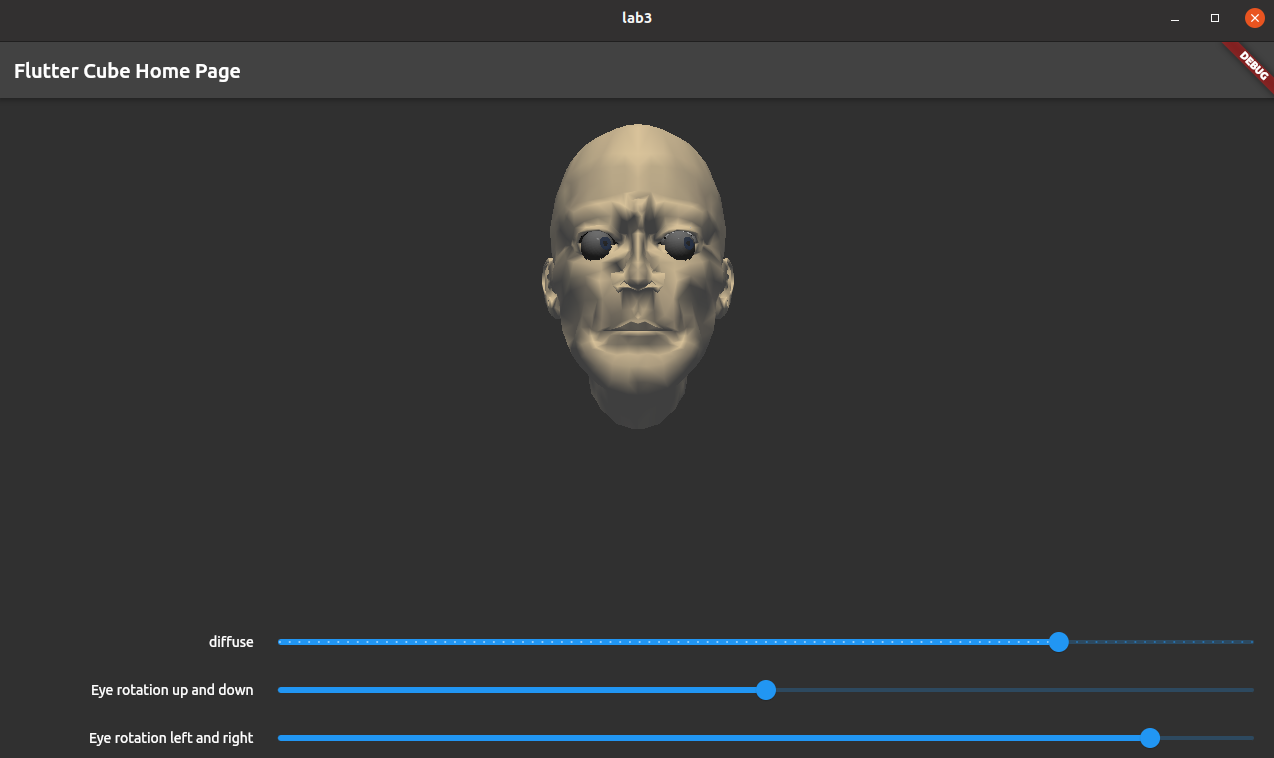
\includegraphics[width=0.8\textwidth]{img2}
\caption{Поворот глаз вправо}
\label{fig:img2}
\end{figure}

\begin{figure}[!htb]
	\centering
	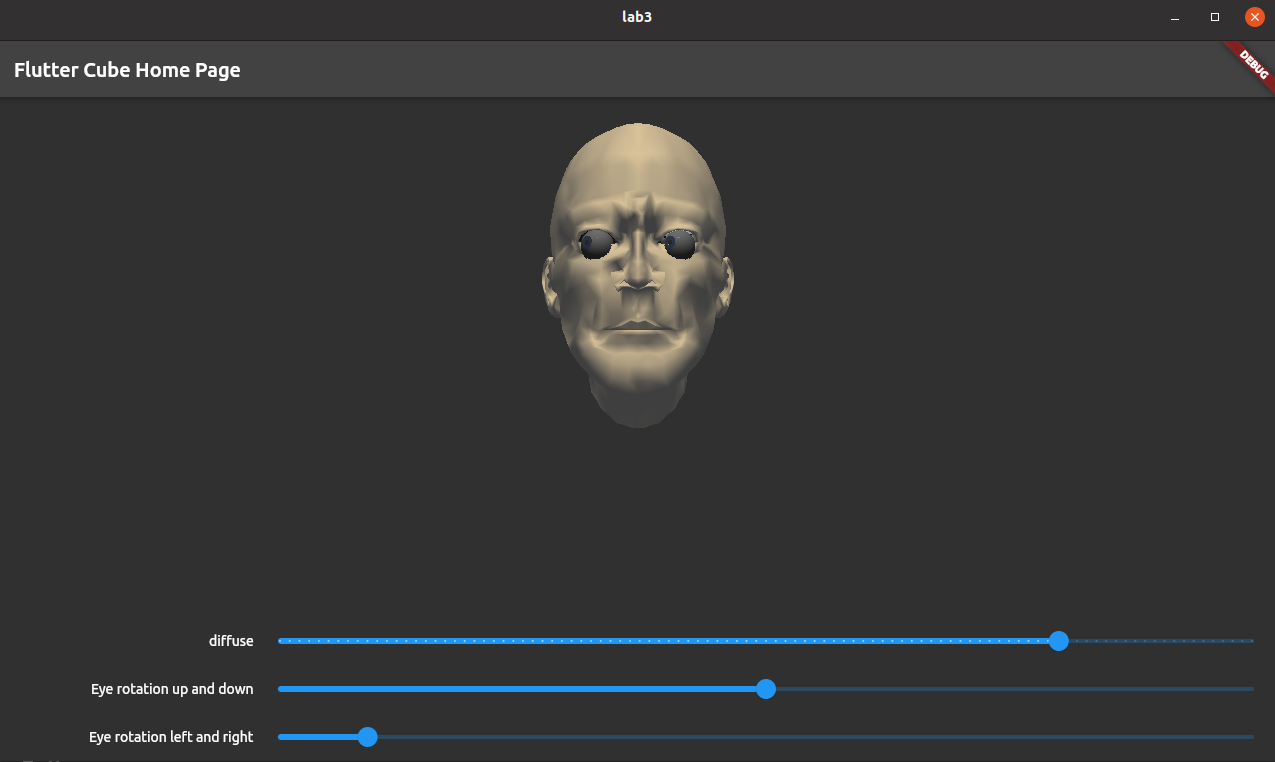
\includegraphics[width=0.8\textwidth]{img3}
\caption{Поворот глаз влево}
\label{fig:img3}
\end{figure}

\begin{figure}[!htb]
	\centering
	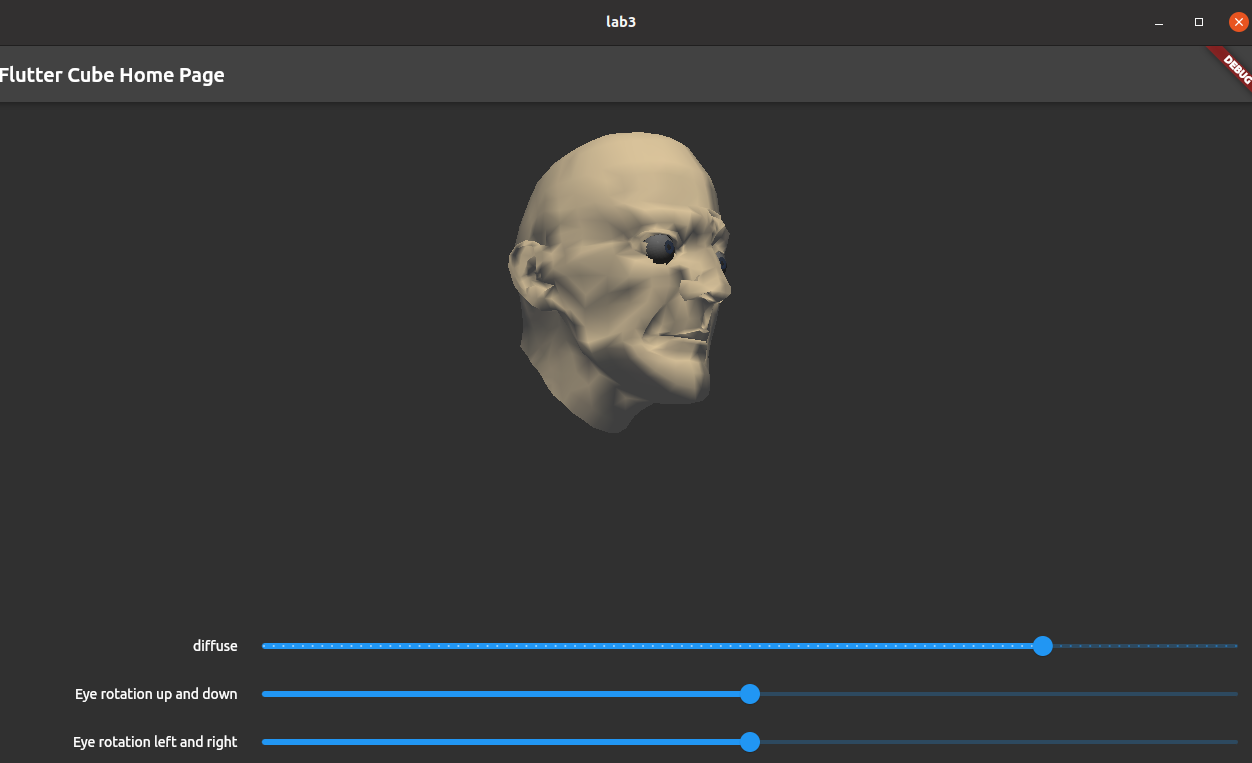
\includegraphics[width=0.8\textwidth]{img4}
\caption{Вращение головы}
\label{fig:img4}
\end{figure}

\section{Выводы}\label{Sect::conclusion}

В результате выполнения лабораторной работы были получены навыки работы с трехмерными объектами, было реализовано приложение моделирования движения глаз человека влево и вправо.

\end{document}